\documentclass{subfiles}

\begin{document}

    \chapter{Planificación}
    \label{chap:planificacion}

        \section{Metodología}
        \label{sec:metodologia}
        
        {Debido a la capacidad de adaptación ante nuevos requisitos y a la posibilidad de generar nuevas entregas a la mayor brevedad posible utilizando metodologías ágiles, se ha optado por esta preferiblemente sobre otras \cite{agilewebsite}. De esta manera, las partes interesadas serían capaces de ver en periodos cortos de tiempo avances en el proyecto que supongan un cambio importante. Es importante mencionar que, debido a que el equipo de desarrollo contaba solamente con una persona, no se ha aplicado el marco de trabajo \textit{Scrum}, puesto que este está planteado para equipos más grandes.}
        
        \paragraph{}
        {Para centrar el trabajo en el menor número de tareas posibles al mismo tiempo, y favorecer la visibilidad del estado de las tareas y del proyecto, se ha decidido utilizar una adaptación de la metodología \Kanban\cite{web:kanban}, una subcategoría de gestión ágil de proyectos centrada en el uso de los tableros homónimos. La idea de usar esta metodología surgió después de atender a una charla de Pablo Santos en la Escuela de Ingeniería Informática en la Universidad de Valladolid \cite{web:pablosantos}, donde nos explicó los diferentes proyectos que dirigió, así como las metodologías que aplicó para liderarlos. En el momento de la charla, explicó como la metodología \Kanban le permitía dar más visibilidad a las tareas en proceso así como ver el flujo de trabajo, tal y como relata en su libro, \textit{Version Control, DevOps and Agile Development with Plastic SCM} \cite{book:santos_pablo_versioncontrol}.}

        \begin{figure}
        \centering
        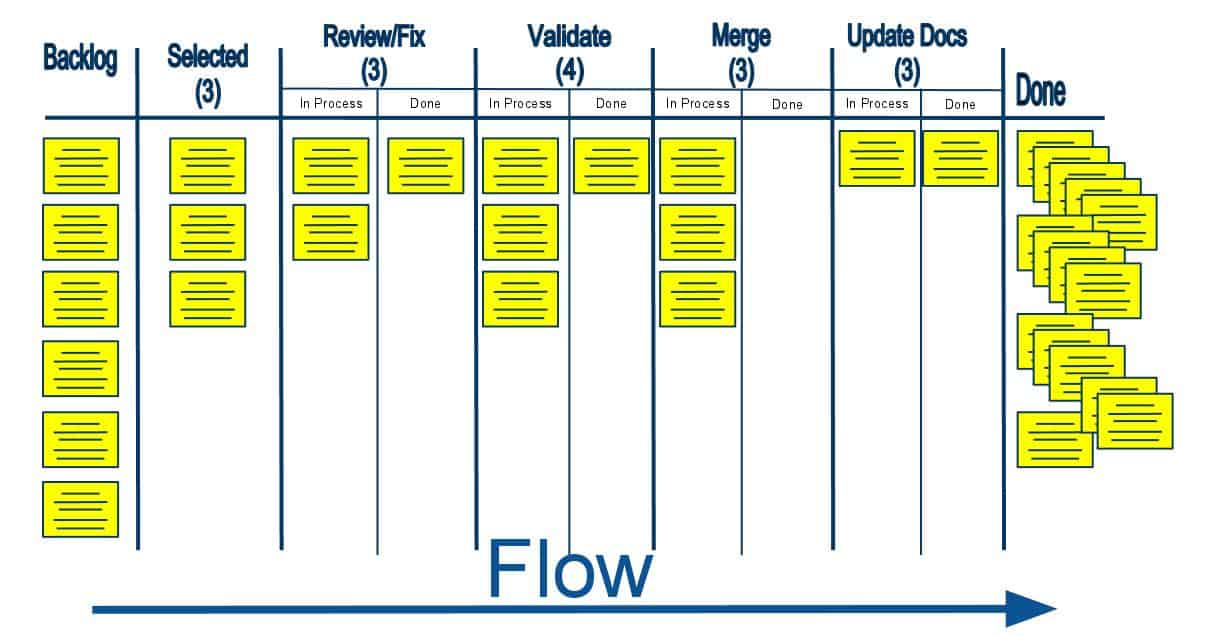
\includegraphics[width=0.8\textwidth]{kanbanboard}
        \caption{Ejemplo de flujo en un tablero \Kanban. Fuente: \citetitle{web:mulesoft_kanban}.}
        \label{fig:kanbanboard}
        \end{figure}

        \paragraph{}
        {Según David Anderson, el ingeniero de Microsoft que aplicó esta metodología por primera vez a proyectos informáticos \cite{book:anderson_david_kanban}, los tableros \Kanban contienen cinco elementos característicos: señales visuales, columnas, límites de trabajo en curso, punto de compromiso y punto de entrega.}

        \begin{itemize}
            \item {\textbf{Señales visuales}: todo el trabajo, junto con su estado actual, debe ser visible de un solo vistazo. Esta metodología utiliza las tarjetas como representación de tareas únicas que, en combinación con las columnas, nos revelarán el flujo de trabajo y el estado actual de este último, todo esto sin abandonar la filosofía de <<información visual>> de \Kanban.}
            \item {\textbf{Columnas}: representan el estado de la tarea en el flujo de trabajo. Los tableros más sencillos suelen utilizar 3 columnas (\textit{pendiente}, \textit{en curso}, \textit{finalizado}), aunque cada equipo puede organizar su flujo de trabajo a placer. Así, para indicar la evolución de cada tarea, las tarjetas avanzarán por diferentes columnas hasta su finalización, yendo idealmente siempre hacia la derecha. En su charla, Pablo Santos llegó a indicar que cada empleado tenía su propia columna de <<trabajo en curso>> para visibilizar de manera más eficaz con qué tarea se encontraba cada empleado.}
            \item {\textbf{Límites de trabajo en curso}: las columnas que indican el trabajo en curso deben tener un límite establecido de tarjetas en ella. Este, según las buenas prácticas, suele ser menor que el número de miembros del equipo para que, si un miembro termina una tarea y no puede comenzar otra por este límite, se dedique a la revisión de código o a apoyar a otros compañeros a finalizar tareas que puedan haberse atascado. Así, cuando una de estas columnas alcanza su límite de tarjetas, el equipo debe aplicar todo su esfuerzo en estas para lograr que avancen. Esta es la forma visual que tiene \Kanban de mostrar al equipo que se está intentando asumir demasiado trabajo y de avisar de posibles cuellos de botella.}
            \item {\textbf{Punto de compromiso}: \Kanban trabaja con una pila de tareas por desarrollar, comúnmente llamada \textit{backlog}, que va creciendo según van apareciendo nuevas necesidades o requisitos. Cada vez que una de esas tareas sale de la columna de tareas pendientes, el miembro del equipo se <<compromete>> a terminar esa tarea en el menor tiempo posible. El momento de inicio de cada tarea se denomina por esto <<punto de compromiso>>}
            \item {\textbf{Punto de entrega}: es el momento en que una tarjeta se convierte en un trabajo completado y, por tanto, está ya en manos del cliente o del producto final. El tiempo entre el punto de compromiso y el punto de entrega se denomina <<plazo>>, y la intención de la forma de trabajar con \Kanban es que ese plazo sea el menor posible.}
        \end{itemize}
        
        \paragraph{}
        {Al ser un proyecto de innovación dentro de la empresa, los requisitos iban surgiendo según íbamos encontrando nueva información al respecto. De esta manera, durante reuniones semanales se comentaba el avance del proyecto, así como las nuevas tareas a incorporar junto con su prioridad, procurando siempre no solapar unas tareas con otras. Esto implica que, al final de dichas reuniones, generalmente se ampliaba el \textit{backlog} del tablero \Kanban, siendo común que en cada reunión surgiesen una o dos nuevas tarjetas. En este aspecto, la aplicación de esta metodología se ajustaba mejor que otras metodologías al trabajo realizado, debido a que toda tarea terminada podía ser subida en <<su propia \textit{release}>>. En ese aspecto, \textit{Scrum} es mucho más estricto, dependiendo de \textit{sprints}. Esta última además es muy dependiente de reuniones (planificaciones de \textit{sprints}, reuniones diarias, revisiones de \textit{sprints}, retrospectivas), que parecen perder utilidad cuando el equipo está reducido a tres personas que, además, mantienen el contacto en todo momento. Se planteó también utilizar un modelo de prototipado de Software, debido a que se desconocía el resultado del producto final y de los requisitos del proyecto. Sin embargo, la investigación previa de los sistemas existentes permitió aclarar muchos aspectos del producto y establecer un plan de ruta que, aunque se pudiese desviar, permitiría planear con mayor o menor antelación las tareas necesarias.}

        \paragraph{}
        A pesar de que no había roles específicos definidos dentro del propio proyecto, sí podían diferenciarse algunos relacionados con la gestión de proyectos asociados a los tres miembros del equipo:
        \begin{itemize}
            \item \textbf{Álvaro Aparicio} procuraba que el desarrollo del producto fuese en todo momento beneficioso para la empresa, dando una serie de ideas generales para que el resto del equipo las diese forma y las llevara a la práctica. Él se dedicaba también a informar al CEO de la empresa de los avances, así como de tratar con otros sectores en caso de necesitar información o ayuda. Su rol sería, en este equipo, el \textit{Product Owner}.
            
            \item \textbf{Alberto Sáenz} tomaba decisiones sobre avances, procuraba hacer de puente entre las ideas generales propuestas por el primer miembro y las tareas técnicas a desarrollar y gestionaba y coordinaba el proyecto así como sus tiempos. Por su implicación, su rol sería \textit{Project Manager}, aunque también haría las veces de \textit{Team Lead} debido a su gestión del trabajo de los miembros.
            
            \item Por último, \textbf{mi posición}, dedicada principalmente al desarrollo, a aprender sobre las nuevas tecnologías y a investigar sobre las mismas, se acercaría principalmente al rol de desarrollador, pero al ser necesario un conocimiento intensivo de las tecnologías aplicadas y su interpretación para el resto del equipo, también se podría aplicar \textit{Tech lead}.
        \end{itemize}

\end{document}